\documentclass[12pt,twoside]{article}
\usepackage{jmlda}
\bibliographystyle{utf8gost705u}
%\NOREVIEWERNOTES
\title
    [Обучение машинного перевода без параллельных текстов] % Краткое название; не нужно, если полное название влезает в~колонтитул
    {Обучение машинного перевода без параллельных текстов}
\author
    [Артеменков~А.\,А$^1$. Гончаров~М.\,Ю.$^1$ Ярошенко~А.\,М.$^1$  Иванов~А.\,В.$^1$ Мазуров~М.\,М.$^1$ Борисова~А.\,В.$^1$ Скиднов~Е.\,А.$^1$ Строганов~А.\,А.$^1$ Рябов ~Ф.\,А.$^1$] % список авторов для колонтитула; не нужен, если основной список влезает в колонтитул
{Артеменков~А.\,А. Гончаров~М.\,Ю. Ярошенко~А.\,М.  Иванов~А.\,В. Мазуров~М.\,М. Борисова~А.\,В. Скиднов~Е.\,А. Строганов~А.\,А. Рябов ~Ф.\,А.} % основной список авторов, выводимый в оглавление
[Артеменков~А.\,А. Гончаров~М.\,Ю. Ярошенко~А.\,М.  Иванов~А.\,В. Мазуров~М.\,М. Борисова~А.\,В. Скиднов~Е.\,А. Строганов~А.\,А. Рябов ~Ф.\,А.] % список авторов, выводимый в заголовок; не нужен, если он не отличается от основного
\thanks
    {Научный руководитель:  Стрижов~В.\,В. 
   Авторы: А.В. Грабовой, О.Ю. Бахтеев, В.В. Стрижов, Eric Gaussier, координатор Малиновский~Г.\,С.
   Консультант:  Бахтеев~О.\,Ю.}
%\email
%    {author@site.ru}
\organization
{Московский физико-технический институт}
\abstract
{В данной работе исследуется задача машинного перевода между двумя языками. Для решения часто используются параллельные предложения, то есть совпадающие по смыслу фразы на двух языках. В работе рассматривается альтернативная модель, не требующая большого количества параллельных предложений. Она использует нейронную сеть типа Seq2Seq, имеющую скрытое пространство. Для проверки качества модели проводится вычислительный эксперимент по переводу предложений между близкими языками, такими как русский и украинский.

\bigskip
\textbf{Ключевые слова}: \emph {нейронные сети, машинный перевод, автокодировщики}.}
\begin{document}
\maketitle

\section{Введение}

В зависимости от специфики пары языков выделяют несколько подходов к машинному переводу. При наличии достаточного числа параллельных предложений(порядка миллиона) использование глубоких нейронных сетей привело к получению хороших результатов \cite{zou2013bilingual},\cite{cho2014properties}. 

Но для многих пар языков нет достаточной базы примеров. Одним из подходов на основе параллельных предложений является пополнение обучающей выборки переводами с предыдущих итераций работы нейронной сети \cite{bertoldi2009domain}. 

Ниже представлено решение задачи машинного перевода при отсутствии достаточного количества параллельных предложений \cite{wu2016google}, \cite{sutskever2014sequence}, \cite{bahdanau2014neural}. В модели используются 2 типа автокодировщиков: рекуррентные нейронные сети \cite{gers1999learning}, \cite{graves2005framewise}, которые реализуют перевод слов в скрытое пространство, и сеть-дискриминатор, определяющая по векторному представлению язык исходного предложения. Сети-энкодеры оптимизируются так, чтобы представление одного и того же предложения на разных языках совпадало в скрытом пространстве, то есть, чтобы дискриминатору было сложнее определить язык, к которому относится вектор. Обучение состоит из двух фаз. На первой оптимизируется работа дискриминатора: предложение кодируется с добавлением шума \cite{kimimproving} и подаётся на вход и происходит перераспределение параметров. На второй стадии происходит перераспределение парамтеров уже у сетей-кодировщиков. После проведение этих шагов вычисляется значение функции потерь. 
 
Такой подход был использован в \cite{lample2017unsupervised} для пары языков французский-английский. В данной работе будет проведен схожий эксперимент для перевода с русского на украинский. Качество переводчика в работе оценивается с помощью метрики BLEU \cite{papineni2002bleu}.

\section{Постановка задачи}
Даны обучающая выборка $\mathfrak{D}^{\text{src}} = \{\mathbf{s}_1^{\text{src}}, \dots, \mathbf{s}_{m_\text{src}}^{\text{src}}\}$, $\mathfrak{D}^{\text{tgt}} = \{\mathbf{s}_1^{\text{tgt}}, \dots, \mathbf{s}_{m_\text{tgt}}^{\text{tgt}}\}$, которая состоит из двух корпусов произвольных предложений для каждого языка; и валидационная выборка $\mathfrak{D}^{valid} = \{(\mathbf{\tilde{s}}_1^{\text{src}}, \mathbf{\tilde{s}}_1^{\text{tgt}}), \dots, (\mathbf{\tilde{s}}_{m_{\text{valid}}}^{\text{src}}, \mathbf{\tilde{s}}_{m_{\text{valid}}}^{\text{tgt}})\}$, которая состоит из пар параллельных предложений.

Задача состоит в том, чтобы, используя обучающую выборку, построить модель $M$ перевода предложений c языка src на язык tgt и выбрать ее параметры таким образом, чтобы максимизировать среднее значение метрики BLEU на валидационной выборке 
$$
\frac{1}{m_{\text{valid}}} \sum_{i=1}^{m_{\text{valid}}} \text{BLEU}(M(\mathbf{\tilde{s}}_i^{\text{src}}), \mathbf{\tilde{s}}_i^{\text{tgt}}) \to \max_{M}
$$ 

\subsection{Гипотеза}
Пусть $\mathcal{S}^{l}$ -- множество всех предложений на языке $l \in \{\text{src}, \text{tgt}\}$. Выдвигается гипотеза о том, что существует единое латентное пространство $\mathcal{L}$ и отображения $\textbf{\textit{f}}^{l}: \mathcal{S}^{l} \to \mathcal{L}$ и $\textbf{\textit{g}}^{l}: \mathcal{L} \to \mathcal{S}^{l}$ такие, что 
\begin{itemize}
	\item для $\forall l_1, l_2 \in \{\text{src}, \text{tgt}\}$ и $\forall s^{l_1} \in \mathcal{S}^{l_1}$ $\textbf{\textit{g}}^{l_2}(\textbf{\textit{f}}^{l_1}(s^{l_1}))$ совпадает с $s^{l_1}$, если $l_1$ совпадает с $l_2$, и является корректным переводом $s^{l_1}$, если $l_1$ и $l_2$ различаются
	%\item для $\forall l \in \{\text{src}, \text{tgt}\}$ и $\forall \mathbf{s}^{l} \in \mathcal{S}^{l}$ $\textbf{\textit{g}}^{l}(\textbf{\textit{f}}^{l}(\mathbf{s}^{l})) = \mathbf{s}^{l}$
	
	%\item для $\forall (l_1, l_2) \in \{(\text{src}, \text{tgt}), (\text{tgt}, \text{src})\}$ $\forall \mathbf{s}^{l_1} \in \mathcal{S}^{l_1}$ $\textbf{\textit{g}}^{l_2}(\textbf{\textit{f}}^{l_1}(\mathbf{s}^{l_1}))$ является корректным переводом $s^{l_1}$ на язык $l_2$
	
	\item распределения образов $\textbf{\textit{f}}^{\text{src}}(\mathcal{S}^{\text{src}})$ и $\textbf{\textit{f}}^{\text{tgt}}(\mathcal{S}^{\text{tgt}})$ совпадают
\end{itemize}

\subsection{Описание метода}
Предлагаемый метод заключается в том, чтобы для каждого $l \in \{\text{src}, \text{tgt}\}$  моделировать отображения $\textbf{\textit{f}}^{l}$ и $\textbf{\textit{g}}^{l}$ кодировщиком $\textbf{f}^{l}$ и декодировщиком $\textbf{g}^{l}$ соответственно. Таким образом, моделью перевода является композиция $\textbf{g}^{\text{tgt}} \circ \textbf{f}^{\text{src}}$. 

Оптимизация проводится следующим образом. Функция ошибки содержит три слагаемых, которые соответствуют сделанным предположениям об отображениях $\textbf{\textit{f}}^{l}$ и $\textbf{\textit{g}}^{l}$.
\paragraph{Ошибка восстановления} Для каждого $l \in \{\text{src}, \text{tgt}\}$ рассматривается входное предложение $\mathbf{s}^{l}$ на языке $l$. Ошибки считаются между $\mathbf{s}^{l}$ и его образом при отображении $\textbf{g}^{l} \circ \textbf{f}^{l}$.

\paragraph{Ошибка перевода} Рассматривается предложение $\mathbf{s}^{\text{src}}$ без ограничения общности на языке src. В качестве входного предложения используется $\mathbf{s}^{\text{tgt}}$ -- перевод $\mathbf{s}^{\text{src}}$, полученный с помощью некоторой слабой модели перевода $M^0$. Ошибка перевода с языка tgt на язык src считается между $\mathbf{s}^{\text{src}}$ и образом $\mathbf{s}^{\text{tgt}}$ при отображении $\textbf{g}^{\text{src}} \circ \textbf{f}^{\text{tgt}}$. Аналогичным образом считается ошибка перевода с языка src на язык tgt. В качестве $M^0$ используется пословный переводчик на основе предобученных векторных представлений слов $\mathcal{E}^{\text{src}} = \{\textbf{x}_i\}_{i=1}^{n_{\text{src}}}$ и $\mathcal{E}^{tgt} = \{\textbf{y}_i\}_{i=1}^{n_{\text{tgt}}}$. Переводом слова $\textbf{x} \in \mathcal{E}^{\text{src}}$ является $\textbf{y} = {\arg\min}_{\textbf{y} \in  \mathcal{E}^{\text{tgt}}} \rho(\textbf{x}, \textbf{y})$, где $\rho$ -- косинусное расстояние (перевод слов языка $\text{tgt}$ осуществляется аналогично).

\paragraph{Штраф за различие распределений} Вводится дискриминатор $\textbf{d}$, который решает задачу классификации векторов $\textbf{h}^l$ латентного пространства $\mathcal{L}$ на классы $\{0, 1\}$: $\textbf{h}^l \in 0 \Leftrightarrow l = \text{src}$. Векторы $\textbf{h}^l$ получаются кодировщиком $\textbf{f}^{l}$, в качестве промежуточного результата при отображениях входных предложений. В функцию ошибки добавляется штраф за то, что дискриминатор точно определяет язык входного предложения. Таким образом параметры модели оптимизируются таким образом, чтобы усложнить задачу дискриминатору. В свою очередь параметры дискриминатора оптимизируются параллельно параметрам модели. Соревновательный процесс оптимизации мотивирован желанием добиться сходства распределений латентных векторов для разных языков.

\subsection{Детали метода}   
Введем словарь $V^{\text{src}}$, содержащий проиндексированные слова, встречающиеся в предложениях из $\mathfrak{D}^{\text{src}}$ и переводах предложений из  $\mathfrak{D}^{\text{tgt}}$, получаемых с помощью $M^0$. Аналогично введем $V^{\text{tgt}}$. 

Предложения на разных языках, использующиеся при оптимизации кодируются с помощью соответствующих словарей. Входные предложения зашумляются преобразованием $\sigma$: сначала с некоторой вероятностью $q$ из них удаляется каждое слово, а затем производится случайная перестановка оставшихся слов с условием, что слово не может оказаться дальше чем на $k$ позиций от своей начальной позиции ($q$, $k$ -- гиперпараметры).

Кодировщик $\textbf{f}^{l}$ включает в себя слой векторного представления слов $\textbf{e}^{l}$, параметры которого инициализируются векторами $\mathcal{E}^{l}$, и реккурентную нейронную сеть $\textbf{r}^{\text{enc}}$. Декодировщик $\textbf{g}^{l}$ включает в себя $\textbf{e}^{l}$, $\textbf{r}^{\text{dec}}$ и классификатор $\textbf{c}^{l}$, который решает задачу многоклассовой классификации выходов $\textbf{r}^{\text{dec}}$ на классы, соотвествующие словам в словаре $V^{l}$ (отображает выходы $\textbf{r}^{\text{dec}}$ в векторы вероятностей размерности $|V^{l}|$). Параметры $\textbf{r}^{\text{enc}}$ и $\textbf{r}^{\text{dec}}$ общие для $\textbf{f}^{\text{src}}$, $\textbf{f}^{\text{tgt}}$ и $\textbf{g}^{\text{src}}$, $\textbf{g}^{\text{tgt}}$ соответственно.

В качестве меры ошибок классификации используется кросс-энтропия $CE$. Итоговый вид функции ошибки

$$
L_{\text{tran}} = w_1 \cdot \sum_{l \in \\ \{src, tgt\}} CE(\textbf{g}^{l}(\textbf{f}^{l}(\sigma(\mathbf{s}^{l}))), \mathbf{s}^{l})\ +
$$
$$
+\ w_2 \cdot \sum_{l_1 \ne l_2 \in \\ \{src, tgt\}} CE(\textbf{g}^{l_2}(\textbf{f}^{l_1}(\sigma(\mathbf{s}^{l_1}))), \mathbf{s}^{l2}) +
w_3 \cdot \sum_{l \in \\ \{src, tgt\}} CE(\textbf{d}(\textbf{f}^{l}(\sigma(\mathbf{s}^{l}))), \mathbb{I}[l = \text{src}])
$$

$$
L_{\text{disc}} = \sum_{l \in \{src, tgt\}} CE(\textbf{d}(\textbf{f}^{l}(\sigma(\mathbf{s}^{l}))), \mathbb{I}[l = \text{tgt}]).
$$

\section{Результаты экспериментов}

В качестве параллельного корпуса была взята выборка на основе OpenSubtitles-2018, в качестве непараллельной выборки - мультиязычные статьи из википедии. Работа была проделана на англо-французской выборке, так как качество найденных русско-украинских выборок не является достаточным как для построения хорошей модели, так и для валидации: в предложениях присутствует слишком много слов не из словаря (числа и формы слов), а сами переводы не всегда точны. Ниже представлены графики зависимости BLEU от номера итерации при различных размерах обучающей выборки и различной размерности скрытого пространства $\mathcal{L}$. Можно сделать вывод, что из-за увеличения числа предложений в обучающей выборке BLEU растёт более медленно, но при этом мы теряем некоторую часть информации о распределении предложений, и ограничиваем максимально достижимое качество. Кроме того, при увеличении размера скрытого пространства модель оптимизируется быстрее, однако при этом повышается риск переобучения.

\begin{figure}[h]
	\centering
	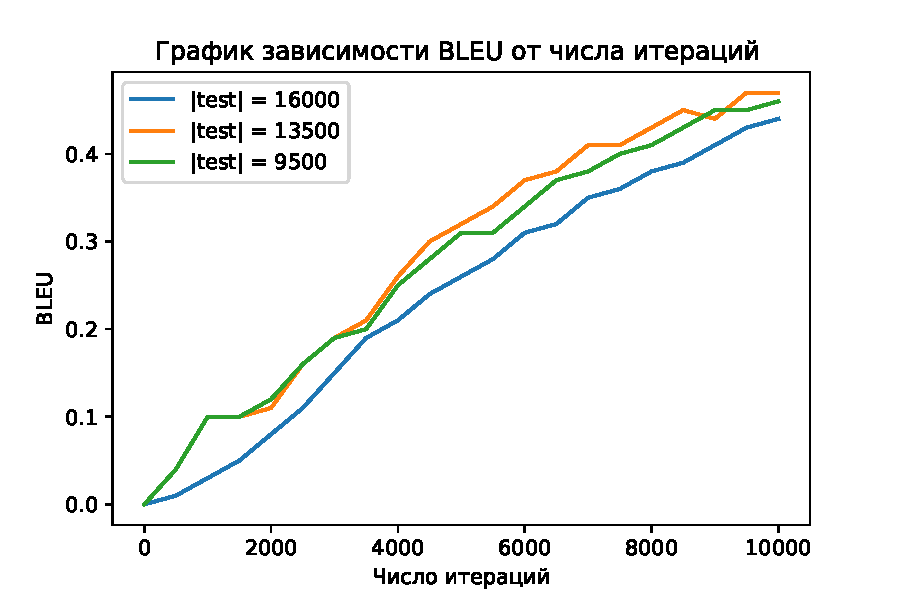
\includegraphics[width=0.7\textwidth]{volume}
	\caption{Зависимость BLEU от размера обучающей выборки.}
\end{figure}

\begin{figure}[h]
	\centering
	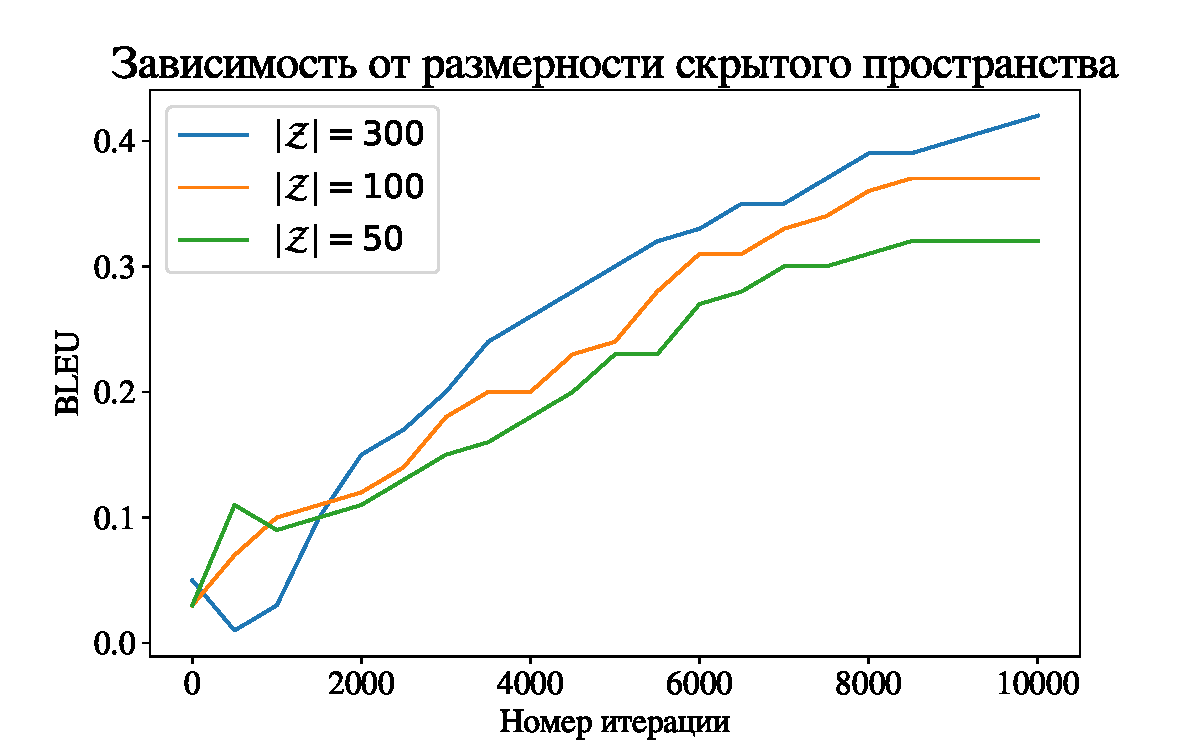
\includegraphics[width=0.7\textwidth]{hidden}
	\caption{Зависимость BLEU от размерности скрытого пространства.}
\end{figure}

\section{Вывод}

В данной работе была исследована задача машинного перевода между двумя языками. Предложен подход, основанный на моделях автокодировщиков и не требующий наличия большого корпуса параллельных предложений. Возможна дальнейшая работа по модификации алгоритма таким образом, чтобы это не так сильно влияло на качество перевода \cite{irvine2016end}, \cite{klementiev2012toward}. В данных работах предлагается извлечь дополнительную информацию из выборки для одного языка, что позволит сохранить независимость метода от наличия параллельных предложений.

\clearpage
\bibliography{references}

%\linenumbers

% Решение Программного Комитета:
%\ACCEPTNOTE
%\AMENDNOTE
%\REJECTNOTE
\end{document}
